\documentclass[journal]{IEEEtran}
%\documentclass[conference]{IEEEtran}
\IEEEoverridecommandlockouts
% The preceding line is only needed to identify funding in the first footnote. If that is unneeded, please comment it out.

\usepackage{url}
\usepackage{xspace}

\usepackage[Algorithm]{algorithm}
\usepackage{algorithmic}
\usepackage{setspace}

\usepackage{cite}
\usepackage{amsmath,amssymb,amsfonts}
\usepackage{algorithmic}
\usepackage{graphicx}
\usepackage{textcomp}
\usepackage{xcolor}
\usepackage{tabularx}

\usepackage{multirow}
\usepackage{booktabs}

\usepackage[spanish]{babel}
\usepackage[utf8]{inputenc}



%paquete para mostrar código
\usepackage{listings}
\usepackage{caption}
\lstset{
	basicstyle=\ttfamily\scriptsize, 
	columns=fullflexible, 
	%numbers=left, 
	%numberstyle=\tiny, 
	%numbersep=5pt,
	framexleftmargin=15pt,
	%framexrightmargin=17pt,
	framexbottommargin=2pt,
	framextopmargin=2pt,
	xleftmargin=15pt,
	frame=top,frame=bottom,
	captionpos=t,
	}

\captionsetup[lstlisting]{singlelinecheck=false, margin=0pt, labelsep=space,labelfont=bf}

%necesario para que diga Listado y no Listing	
\renewcommand{\lstlistingname}{Listado}	

\lstnewenvironment{sflisting}[1][]
{\lstset{#1}}{}

%%ejemplo de estilo para el lenguaje SPARQL

\lstdefinelanguage{sparql}{
	morecomment=[l][\color{teal}]{\#},
	morestring=[b][\color{blue}]\",
	morekeywords={SELECT,CONSTRUCT,DESCRIBE,ASK,WHERE,FROM,NAMED,PREFIX,BASE,OPTIONAL,FILTER,GRAPH,LIMIT,OFFSET,SERVICE,UNION,EXISTS,NOT,BINDINGS,MINUS,a,as,GROUP,BY,SUM,AVG,VALUES},
	sensitive=false
}

%listings styles
\lstdefinestyle{sparql}{
	basicstyle=\ttfamily\scriptsize, 
	language=sparql,
	columns=fullflexible, 
	numberstyle= \tiny, %\scriptsize,
	numbers=left,
	frame=lines,
	tabsize=2}

\lstdefinestyle{python}{
	basicstyle=\ttfamily\scriptsize, 
	language=Python,
	columns=fullflexible, 
	numberstyle= \tiny, %\scriptsize,
	%numbers=left,
	frame=lines,
	tabsize=2}


\makeatletter
\newcommand{\linebreakand}{%
\end{@IEEEauthorhalign}
\hfill\mbox{}\par
\mbox{}\hfill\begin{@IEEEauthorhalign}
}
\makeatother


\def\BibTeX{{\rm B\kern-.05em{\sc i\kern-.025em b}\kern-.08em
    T\kern-.1667em\lower.7ex\hbox{E}\kern-.125emX}}
\begin{document}

\title{GraFIng: Base de datos de grafos de la Facultad de Ingeniería de la Universidad de la República}


\author{
	\begin{tabular}{cc}
		\begin{tabular}{c}
			Graciana Castro                                              \\
			\textit{Facultad de Ingeniería, Universidad de la República} \\
			Montevideo, Uruguay                                          \\
			gcastro@fing.edu.uy
		\end{tabular}
		 &
		\begin{tabular}{c}
			Julian O'Flaherty                                            \\
			\textit{Facultad de Ingeniería, Universidad de la República} \\
			Montevideo, Uruguay                                          \\
			julian.o.flaherty@fing.edu.uy
		\end{tabular}
	\end{tabular}
}


\maketitle

\begin{abstract}
	El objetivo de este proyecto fue el diseño e implementación de una base de datos de grafos con información sobre individuos de la Facultad de Ingeniería de la Universidad de la República, Uruguay, y sus distintos trabajos. La información fue obtenida mediante \textit{scraping} de los sitios Colibrí\footnote{\url{https://www.colibri.udelar.edu.uy/jspui/}}, el repositorio institucional de la Universidad, y OpenAlex\footnote{\url{https://openalex.org/}}. Se implementó un grafo de propiedades y las consultas se realizaron utilizando \textit{Cypher}. Como resultado, se construyó una base de datos flexible que permite analizar relaciones entre autores y trabajos, facilitando consultas complejas y la visualización de la información académica de la institución.
\end{abstract}

\section{Introducción}
\label{introduccion}
El análisis de la producción científica y las redes de colaboración académica es una tarea de creciente importancia para las instituciones de investigación. La capacidad de identificar patrones de coautoría, seguir la evolución de líneas de investigación o descubrir conexiones interdisciplinarias aporta valor estratégico a la institución y fortalece a la comunidad científica. Sin embargo, la información académica suele encontrarse dispersa en múltiples repositorios, dificultando una visión integrada. Las bases de datos de grafos ofrecen una estructura adecuada para este desafío, ya que modelan de forma nativa las relaciones entre entidades como autores, publicaciones e instituciones, facilitando consultas que resultan inherentemente complejas en modelos de datos tradicionales.

En este contexto, el objetivo de este proyecto fue el diseño e implementación de una base de datos de grafos para centralizar y estructurar la información sobre los individuos y sus trabajos académicos en la Facultad de Ingeniería (Fing) de la Universidad de la República (UdelaR). Se buscó construir una herramienta que permitiera a investigadores, estudiantes y administradores analizar las redes de conocimiento de la institución de manera ágil e intuitiva.

Por tratarse de un trabajo de fin de curso, el alcance del proyecto se acotó a un subconjunto representativo y manejable del universo de datos. La población de estudio se limitó a los individuos de la Facultad de Ingeniería con trabajos publicados en Colibrí. Para ampliar la cantidad de trabajos de cada persona, se utilizó como fuente secundaria OpenAlex, pero no se incluyeron más individuos.

Este artículo detalla el proceso de construcción de dicha base de datos, desde la extracción de datos hasta la implementación del modelo de grafo, y demuestra su utilidad a través de ejemplos de consulta y análisis. El trabajo se organiza de la siguiente manera: la sección \ref{relacionados} revisa los antecedentes; la sección \ref{desarrollo} describe la metodología de diseño e implementación; la sección \ref{expe} presenta los resultados obtenidos, y finalmente, la sección \ref{conclusion} expone las conclusiones y líneas de trabajo futuro.

\section{Trabajos Relacionados}
\label{relacionados}
Existen antecedentes en el modelado de información académica mediante grafos, como la \textit{dblp computer science bibliography}\footnote{\url{https://dblp.org/}}, una base de datos de publicaciones del área de la informática que estructura la información en un grafo RDF. Su enfoque sirvió como modelo conceptual para nuestro sistema. Una inspiración directa fue el trabajo de fin de curso "El número Abreu" \cite{abreu2023}, realizado en 2023 para la asignatura Bases de Datos no Relacionales, que implementó la exploración de redes de jugadores de futbol y motivó la ejecución de una red similar para la comunidad académica de la Fing.

\section{Parte central}
\label{desarrollo}
En esta sección se describe el proceso de diseño e implementación de la base de datos de grafos, detallando las decisiones tomadas y los pasos seguidos.

\subsection{Obtención y Preprocesamiento de Datos}
El primer paso del proyecto fue la recolección de datos. Para ello, se desarrollaron herramientas de extracción automatizada (\textit{scraping}) en Python, organizadas en el módulo \texttt{udelar\_graph/extraction}. Las fuentes utilizadas fueron Colibrí y OpenAlex.

Colibrí es el \textit{``repositorio institucional de la Universidad de la República''}, donde se pueden encontrar proyectos de fin de carrera, tesis, artículos de investigación, entre otros. Para obtener los registros del mismo se implementó un scraper utilizando la librería de Python \emph{Scrapy}~\cite{scrapy} que recorrió las páginas del repositorio, identificó los registros relevantes en el HTML y los guardó en formato \emph{JSONL}.
Posteriormente, estos archivos fueron procesados para extraer información estructurada como autores, títulos y afiliaciones. El primer inconveniente que se encontró fue la existencia de autores duplicados con nombres similares, por ejemplo, \textit{Etcheverry, Lorena}, \textit{Echeverry, L} y \textit{Etcheverry Venturini, Lorena}. Para resolver este problema, se implementó un algoritmo de agrupamiento de nombres a base de heurísticas para hacer una primera reducción, y luego se utilizó un modelo de lenguaje (\emph{GPT-4o-mini}) para obtener un nombre y apellido para cada grupo de nombres. Este último paso de estructuración permite reducir aún más la cantidad de duplicados en el grafo y es útil para la conexión con los datos extraídos de OpenAlex.

OpenAlex~\cite{Priem2022OpenAlex} es un índice que colecta información de publicaciones, autores, instituciones y más, y ofrece la capacidad de hacer búsquedas sobre la misma. La extracción de datos se realizó de la forma más simple, buscando todos los trabajos asociados con la Universidad de la República y descargando los resultados en formato \emph{CSV}. Para poder filtrar solo los trabajos asociados a investigadores y estudiantes de la Fing, se supuso que toda persona afiliada a la Fing tiene al menos un registro en Colibrí. Con esta hipótesis, se realizó un matcheo de nombres entre personas de ambas fuentes y se descartaron todos los trabajos que no tuvieran afiliados en la Fing. En la Tabla~\ref{tab:datos} se puede ver el resumen de los datos obtenidos de ambas fuentes.

\begin{table}[h]
	\centering
	\begin{tabular}{l|c|c|c|c}
		\toprule
		\textbf{Fuente} & \textbf{Personas} & \textbf{Trabajos} & \textbf{Autorías} & \textbf{Tutorías} \\
		\midrule
		Colibrí         & 5173              & 3974              & 11180             & 3398              \\
		OpenAlex        & -                 & 8123              & 14596             & -                 \\
		\midrule
	\end{tabular}
	\caption{Resumen de los datos de personas y trabajos obtenidos de las fuentes.}
	\label{tab:datos}
\end{table}

\subsection{Modelado y Carga del Grafo}
Para el modelado se optó por un grafo de propiedades, gestionado con la base de datos Neo4j. En este modelo, los nodos representan entidades (Personas, Trabajos, Tipos de Trabajo y Palabras Clave) y las relaciones modelan los vínculos entre ellas (autoría, contribución, tipo y palabra clave). La Figura~\ref{fig:grafo} ilustra el esquema del grafo implementado.

\begin{figure}[htb]
	\centering
	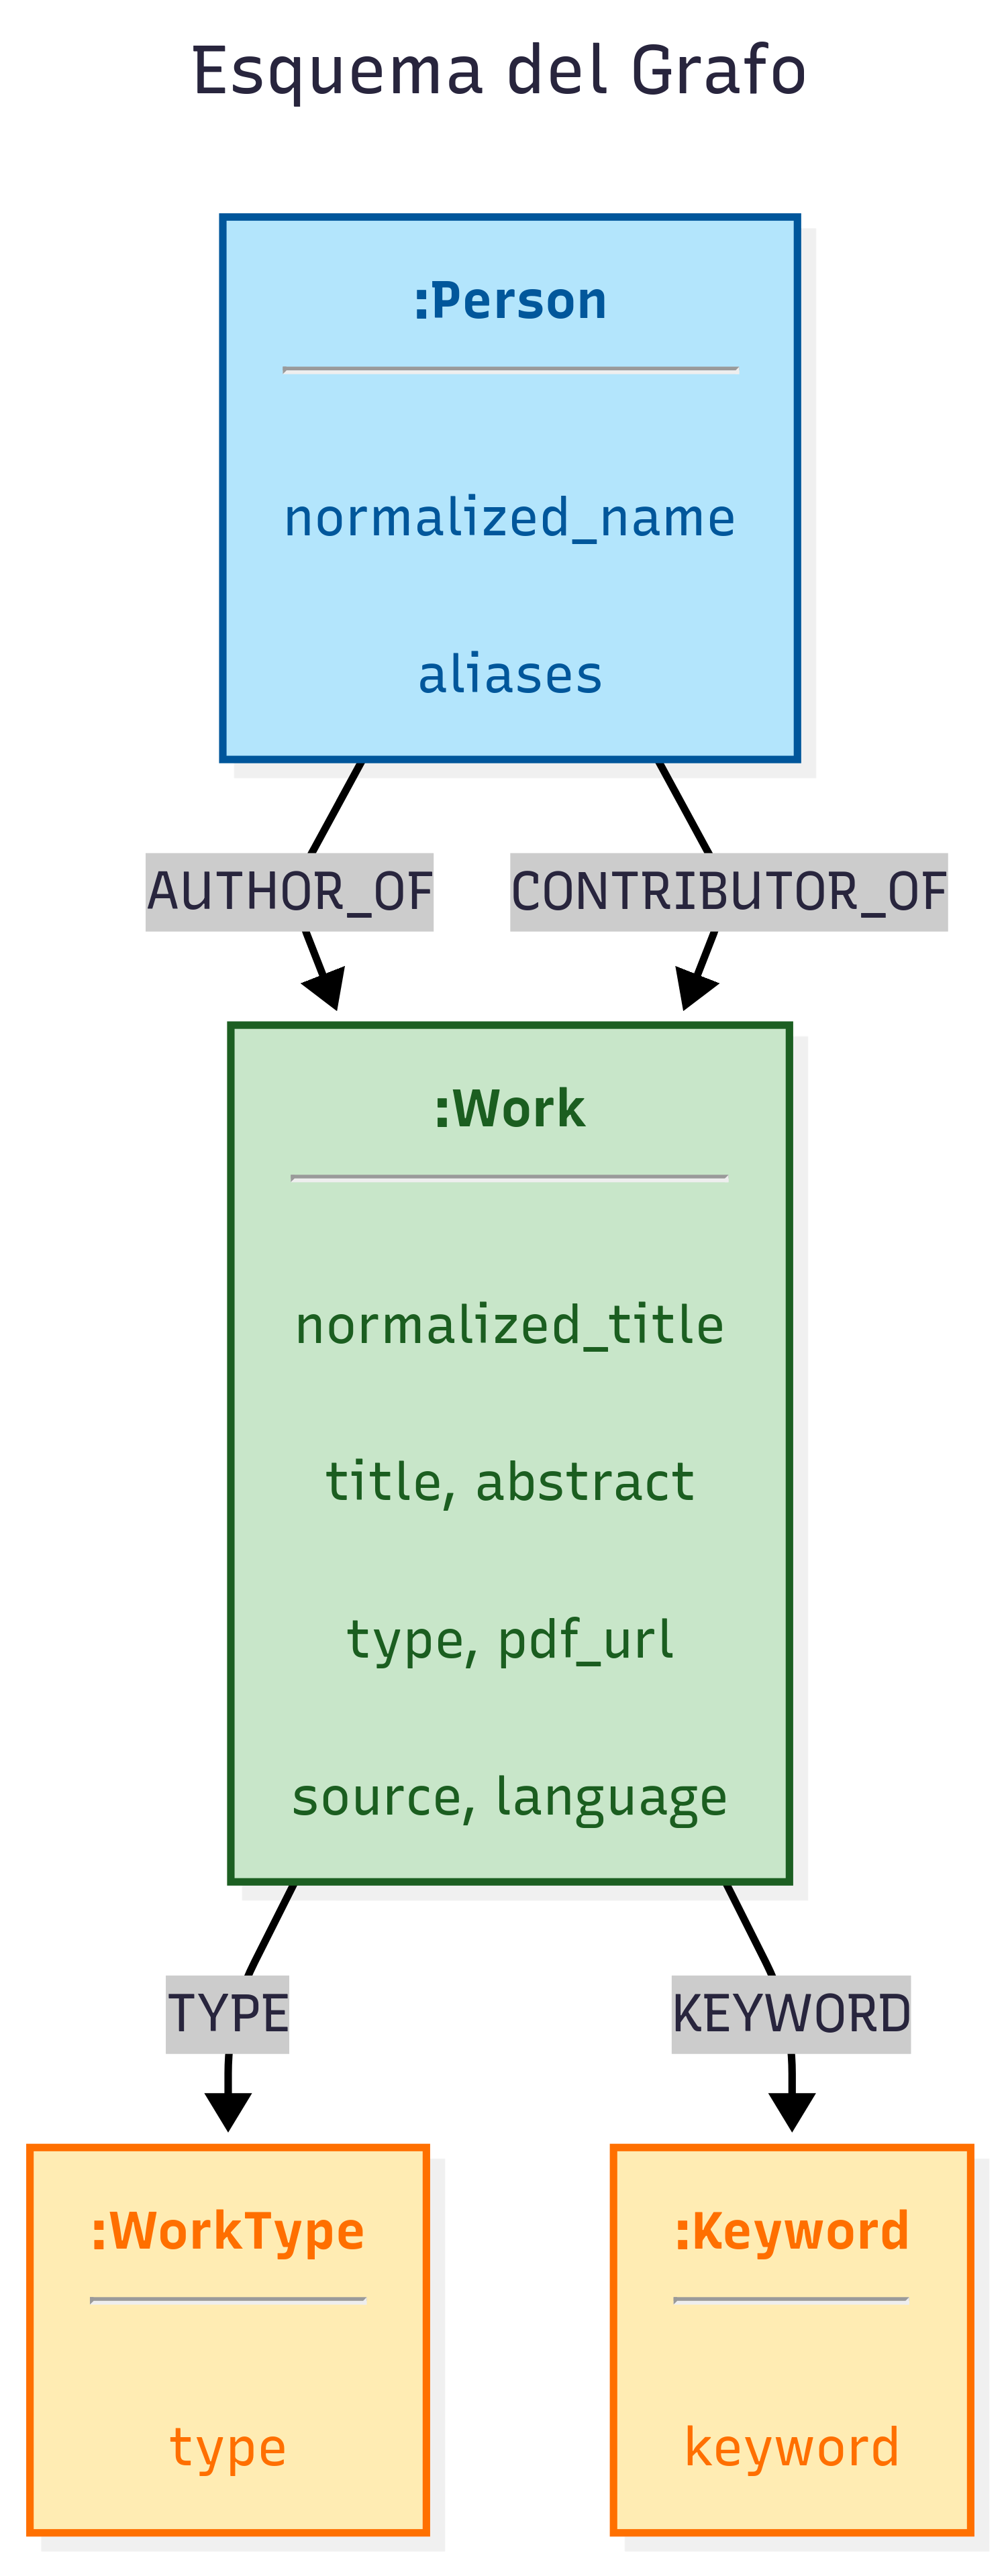
\includegraphics[width=0.6\linewidth]{imagenes/grafo.png}
	\caption{Esquema del grafo de propiedades implementado.}
	\label{fig:grafo}
\end{figure}
Los nodos de tipo \texttt{PERSON} representan a los individuos de la Fing, incluyendo docentes, estudiantes e investigadores. Los nodos \texttt{WORK} almacenan información sobre los trabajos académicos, que tienen definido el tipo con la relación \texttt{TYPE} con los nodos \texttt{WORK\_TYPE}. Se clasifican según su naturaleza en artículo, tesis, tesis de maestría, etc. Los nodos \texttt{KEYWORD} almacenan palabras clave asociadas a cada trabajo.
La relación \texttt{AUTHOR\_OF} conecta a los investigadores con los artículos que han escrito y a los estudiantes con sus tesis. La relación \texttt{CONTRIBUTOR\_OF} permite registrar aquellos docentes que fueron tutores de una tesis.

La carga de los datos se automatizó mediante scripts de Python que utilizan la biblioteca oficial de Neo4j. El proceso, encapsulado en el módulo \texttt{udelar\_graph/load/colibri.py}, transforma los datos preprocesados en nodos y relaciones mediante consultas Cypher. Para facilitar la ejecución, se implementó una interfaz de línea de comandos (CLI) con la biblioteca Typer. El comando \texttt{colibri-load} permite poblar la base de datos, incluyendo una opción para limpiarla previamente y así garantizar la reproducibilidad de los experimentos. Una vez cargados los datos de Colibrí, se ejecutó el comando \texttt{openalex-load} para integrar los datos de OpenAlex.

\subsection{Limitaciones}
El desarrollo del sistema enfrentó limitaciones inherentes a las fuentes de datos y al alcance del proyecto. La cobertura de Colibrí no es exhaustiva y presenta inconsistencias en sus metadatos. Aunque la integración con OpenAlex mitigó parcialmente este problema, la correspondencia entre registros no siempre fue directa. Finalmente, la implementación se realizó sobre una instancia local de Neo4j, con las consiguientes restricciones de escalabilidad. Estas limitaciones abren claras oportunidades para trabajo futuro, como la ampliación del conjunto de datos y la mejora de los procesos de limpieza y normalización.

Otra limitante es que el grafo actualmente no incluye información temporal sobre los trabajos, por lo que no pueden evaluarse tendencias o evoluciones en la producción académica.

\section{Experimentación}
\label{expe}
En esta sección se presentan ejemplos de consultas realizadas sobre el grafo, utilizando el lenguaje Cypher, realizadas para validar el modelo y demostrar la utilidad de la base de datos para el análisis de la producción académica. Además, se presenta un análisis de centralidad del grafo y de detección de comunidades.

\subsection{Consultas relevantes}
A continuación se muestran algunos ejemplos de las consultas realizadas sobre el grafo. En este informe se detallarán aquellas consultas que se consideran más relevantes para demostrar la viabilidad y utilidad del grafo. En el repositorio del trabajo\footnote{\url{https://github.com/j-oflaherty/bdnr-proyecto-final}} se encuentra un conjunto más completo de consultas que se pueden realizar.

\subsubsection{Todos los trabajos de una determinada persona}
Es de utilidad conocer toda la producción académica de una persona, para conocer cuál fue su área de especialización a lo largo de su carrera. Para eso, se puede realizar la consulta mostrada a continuación:

\begin{sflisting}[style=sparql,caption= Obtener los trabajos de una persona,label=trabajos_persona]
	MATCH (p:Person {normalized_name: \$person_name})
	-[:AUTHOR_OF]->(w:Work)
	RETURN w
\end{sflisting}

\subsubsection{Persona con mayor cantidad de estudiantes tutoreados}
Puede ser de interés para estudiantes en búsqueda de tutores para su proyecto final de grado, conocer qué docentes poseen experiencia en la tarea. Para eso, se puede consultar a las personas con más estudiantes tutoreados, teniendo en cuenta que se identifican aquellas personas que tutorearon un trabajo con la relación \texttt{CONTRIBUTOR\_OF}. Para obtener el top cinco de docentes con mayor cantidad de estudiantes, se debe realizar la siguiente consulta:

\begin{sflisting}[style=sparql,caption= Docentes con mayor cantidad de estudiantes tutoreados,label=docentes_con_mas_estudiantes]
	MATCH (p:Person)-[:CONTRIBUTOR_OF]->(w:Work)
	<-[:AUTHOR_OF]-(a:Person)
	RETURN p, COUNT(DISTINCT a) AS students_count
	ORDER BY students_count DESC
	LIMIT 5
\end{sflisting}

\subsubsection{\textit{Keywords} más frecuentes}
Identificar las \textit{keywords} más frecuentes puede ser importante para conocer los temas de interés dentro de un centro académico. Para el grafo implementado, esto se puede obtener con la siguiente consulta, con la que se obtienen las veinte \textit{keywords} más utilizadas:

\begin{sflisting}[style=sparql,caption= \textit{Keywords} más frecuentes,label=keywords]
	MATCH (w:Work)-[:KEYWORD]->(k:Keyword)
	WHERE k.keyword <> "None"
	RETURN k, COUNT(w) AS works_count
	ORDER BY works_count DESC
	LIMIT 20
\end{sflisting}

Al ejecutar la consulta, se observa que dos de los conceptos que más aparecen son \textbf{aprendizaje automático} y \textit{\textbf{machine learning}}, lo que muestra la importancia que tiene esta área para la Facultad de Ingeniería.

\subsubsection{Dúo dinámico}
En este caso, la consulta implementada responde a la pregunta: ¿quiénes son las diez parejas con mayor producción académica en conjunto?

\begin{sflisting}[style=sparql,caption= Parejas con mayor cantidad de artículos publicados en conjunto,label=duo_dinamico]
	MATCH (p1:Person)-[]->(w:Work)<-[]-(p2:Person)
	WHERE elementId(p1) < elementId(p2)
	RETURN p1.normalized_name as person1,
	p2.normalized_name as person2,
	count(w) as collaborations
	ORDER BY collaborations DESC
	LIMIT 10
\end{sflisting}

\subsubsection{Camino más corto entre dos personas}
Para analizar una comunidad y sus actores, también es útil poder identificar el camino que hay entre dos de ellos. En este caso, las personas están vinculadas a través de los trabajos de los que fueron parte, ya sea como autores o como tutores. Para esto, se implementó la siguiente consulta que devuelve el camino más corto entre dos personas:

\begin{sflisting}[style=sparql,caption= Camino más corto entre dos personas,label=camino_corto]
	MATCH
	(p1:Person {normalized_name: \$person1}),
	(p2:Person {normalized_name: \$person2}),
	path = shortestPath(
	(p1)-[:AUTHOR_OF|CONTRIBUTOR_OF*1..{max_length}]-(p2)
	)
	RETURN path
\end{sflisting}

La respuesta muestra un camino intercalado de personas y trabajos. La longitud mínima del camino será dos, ya que entre dos personas siempre deberá haber un trabajo en medio (para el caso de coautores).

En la figura \ref{fig:camino_corto} se muestra la respuesta (en un formato que facilita su lectura) que se obtiene al realizar la consulta para obtener el camino más corto entre los autores de este trabajo.

\begin{figure}[htb]
	\centering
	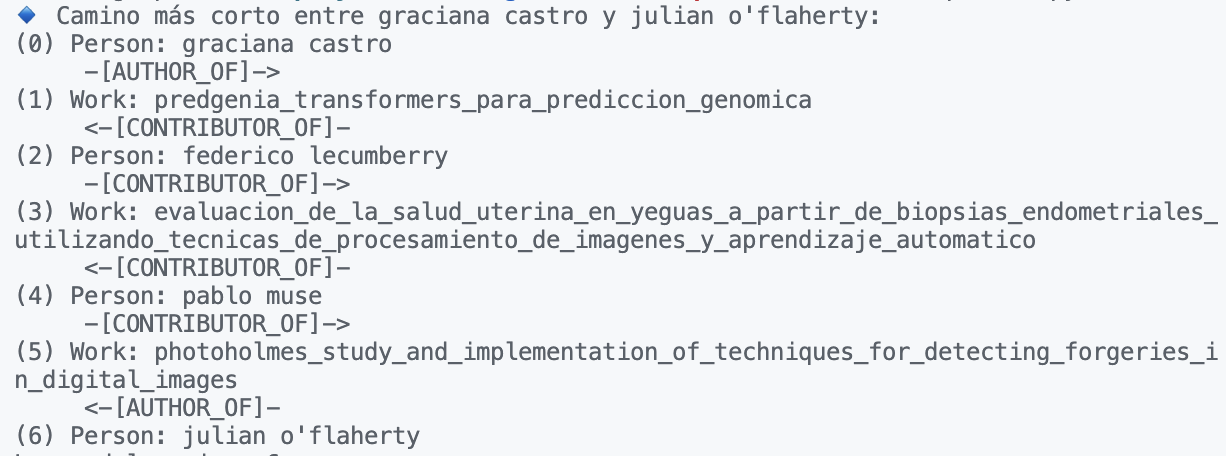
\includegraphics[width=\linewidth]{imagenes/camino_corto.png}
	\caption{Ejemplo de respuesta a la consulta: ``Cuál es el camino más corto entre una persona A (graciana castro) y una persona B (julian o'flaherty)''.}
	\label{fig:camino_corto}
\end{figure}

\subsection{Análisis de centralidad}
En esta sección se presentan las consultas implementadas para el análisis de centralidad del grafo. Para esta tarea, se utilizó el plugin de \textit{graph-data-science}, con el cual se realizó una proyección del grafo con nodos únicamente del tipo \texttt{Person} conectadas entre sí cuando trabajaron en un trabajo en común, con peso igual a la cantidad de trabajos en común.
Esto simplifica la tarea realizada en la última consulta presentada en la sección anterior, en la que para hallar el camino entre dos personas se debía pasar por sus trabajos. En este nuevo grafo, las personas quedan conectadas entre sí directamente. Para esto, debe realizarse la siguiente consulta:

\begin{sflisting}[style=sparql,caption= Consulta para obtener la proyección del grafo de personas,label=subgrafo]
	MATCH (p1:Person)-[:AUTHOR_OF|CONTRIBUTOR_OF]->(w:Work)
	<-[:AUTHOR_OF|CONTRIBUTOR_OF]-(p2:Person)
	WHERE p1 < p2
	WITH p1 as source, p2 as target, count(w) as weight
	WITH gds.graph.project(
		'coauthor-graph',
		source,
		target,
		{relationshipProperties: {weight: weight}},
		{undirectedRelationshipTypes: ['*']}
	) as g
	RETURN g.graphName AS graph, g.nodeCount
	AS nodes, g.relationshipCount AS rels
\end{sflisting}

\subsubsection{Centralidad de Intermediación}

La centralidad de intermediación mide la importancia de un nodo en una red, considerando la cantidad de veces que ese nodo aparece en \textit{el camino más corto entre otras dos personas}. Los nodos con alta centralidad actúan como puentes entre distintas partes del grafo y demuestran una fuerte influencia dentro de la comunidad. Con la siguiente consulta, se obtienen las diez personas con mayor medida de centralidad entre nodos.

\begin{sflisting}[style=sparql,caption= Centralidad de Intermediación,label=intermediacion]
	CALL gds.betweenness.stream('coauthor-graph')
	YIELD nodeId, score
	RETURN gds.util.asNode(nodeId).normalized_name
	AS name, score
	ORDER BY score DESC
	LIMIT 10
\end{sflisting}

En la figura \ref{fig:intermediacion} se muestra la respuesta a la consulta realizada.

\begin{figure}[htb]
	\centering
	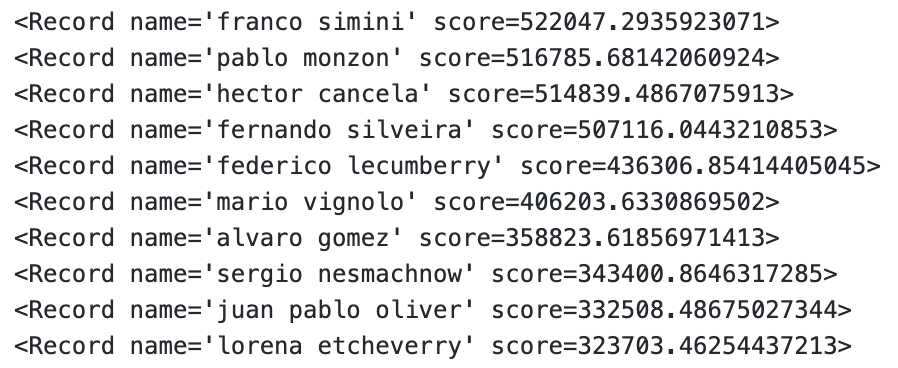
\includegraphics[width=\linewidth]{imagenes/intermediacion.png}
	\caption{Top diez de personas con mayor puntaje de centralidad de intermediación.}
	\label{fig:intermediacion}
\end{figure}

\subsubsection{Centralidad de Cercanía}
La centralidad de cercanía mide qué tan cerca está un determinado nodo del resto de los nodos del grafo. Es importante tener en cuenta que el cálculo de la centralidad de cercanía puede fallar si hay partes del grafo no conectadas, dado que en ese caso la distancia es infinita. Para evitar este problema, se utiliza la normalización de \textit{Wasserman-Faust}, que hace que solo se consideren los nodos alcanzables y luego normaliza el resultado por el tamaño de la componente alcanzada. Para el cálculo de esta centralidad, se realiza la siguiente consulta:

\begin{sflisting}[style=sparql,caption= Centralidad de Cercanía,label=cercania]
	CALL gds.closeness.stream('coauthor-graph',
	{useWassermanFaust: true})
	YIELD nodeId, score
	RETURN gds.util.asNode(nodeId).normalized_name
	AS name, score
	ORDER BY score DESC
	LIMIT 10
\end{sflisting}

Los resultados obtenidos se muestran en la figura \ref{fig:cercania}.

\begin{figure}[htb]
	\centering
	\includegraphics[width=\linewidth]{imagenes/cercanía.png}
	\caption{Top diez de personas con mayor puntaje de centralidad de cercanía.}
	\label{fig:cercania}
\end{figure}

\subsubsection{Centralidad de Grado}

La centralidad de grado puede calcularse ponderada o no ponderada. La no ponderada mide qué nodos tienen más alcance. Por su lado, la ponderada mide aquellos nodos con conexiones más fuertes (en el caso del trabajo, las colaboraciones más repetidas).

La consulta para ambos casos es similar. A continuación se muestra la consulta que se realiza para obtener la centralidad de grado ponderada. Para el caso de la no ponderada, se debe eliminar el parámetro \texttt{{relationshipWeightProperty: 'weight'}}.

\begin{sflisting}[style=sparql,caption= Centralidad de Grado,label=grado_ponderado]
	CALL gds.degree.stream('coauthor-graph',
	{relationshipWeightProperty: 'weight'})
	YIELD nodeId, score
	RETURN gds.util.asNode(nodeId).normalized_name AS name,
	score AS centrality_measure
	ORDER BY centrality_measure DESC, name DESC
	LIMIT 10
\end{sflisting}

La respuesta para la centralidad de grado ponderada se muestra en la figura \ref{fig:grado_ponderada}.

\begin{figure}[htb]
	\centering
	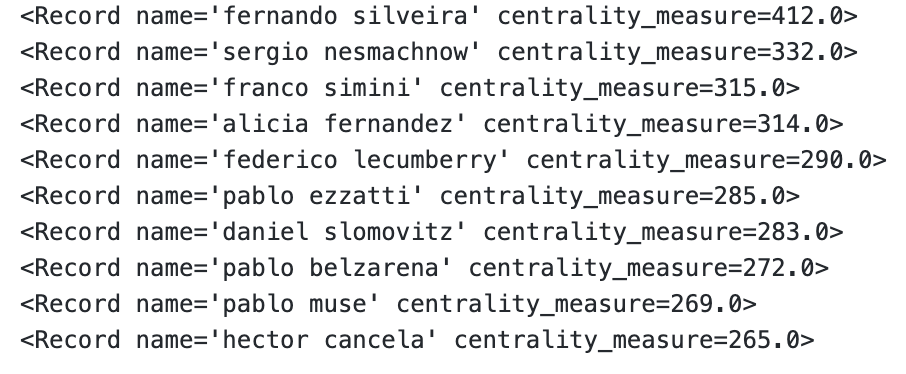
\includegraphics[width=\linewidth]{imagenes/pesos_grado.png}
	\caption{Top diez de personas con mayor puntaje de centralidad de grado ponderada.}
	\label{fig:grado_ponderada}
\end{figure}

\subsubsection{Centralidad de Vector Propio}
La centralidad de vector propio identifica como nodos importantes a aquellos nodos conectados a otros nodos importantes. A continuación se muestra la consulta a realizar y la respuesta en la figura \ref{fig:vector_propio}.
\begin{sflisting}[style=sparql,caption= Centralidad de Vector Propio,label=eigenvector]
	CALL gds.eigenvector.stream('coauthor-graph')
	YIELD nodeId, score
	RETURN gds.util.asNode(nodeId).normalized_name
	AS name, score AS eigenvector
	ORDER BY eigenvector DESC
	LIMIT 10
\end{sflisting}

\begin{figure}[htb]
	\centering
	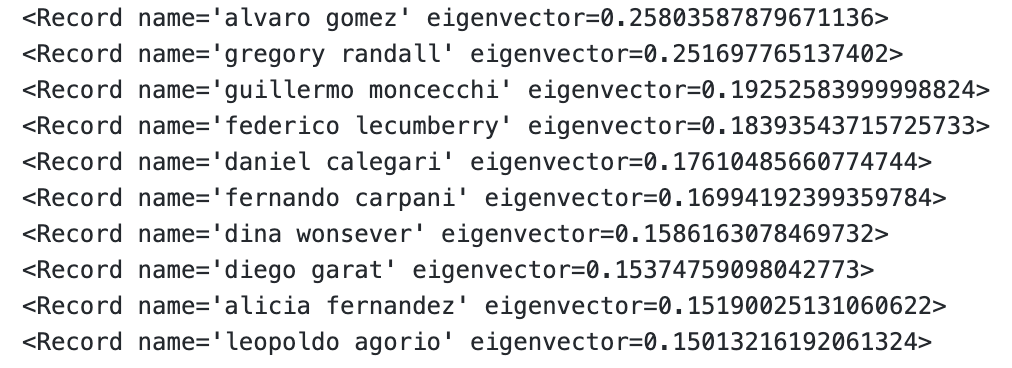
\includegraphics[width=\linewidth]{imagenes/eigenvector.png}
	\caption{Top diez de personas con mayor puntaje de centralidad de vector propio.}
	\label{fig:vector_propio}
\end{figure}

\subsubsection{\textit{PageRank}}
\textit{PageRank} es un algoritmo que mide la importancia de un nodo considerando si otros nodos ``votan'' por él. No solo importa la cantidad de votos, sino también la importancia del nodo que vota. El voto de un nodo muy importante tiene mayor peso que el de uno poco importante. También importa cuántos votos da cada nodo; si un nodo tiene muchas relaciones, cada una de ellas tiene menor peso que las de un nodo con pocas relaciones. En este caso, en que el grafo es no dirigido, cuando dos nodos A y B están relacionados entre sí significa que A vota por B y B vota por A (se toma esa relación como dos relaciones dirigidas).

Para obtener el puntaje de PageRank, se debe realizar la siguiente consulta:

\begin{sflisting}[style=sparql,caption= PageRank,label=pagerank]
	CALL gds.pageRank.stream('coauthor-graph')
	YIELD nodeId, score
	RETURN gds.util.asNode(nodeId).normalized_name
	AS name, score AS pageRank
	ORDER BY pageRank DESC
	LIMIT 10
\end{sflisting}

Se muestra en la figura \ref{fig:page_rank} el resultado de la consulta.

\begin{figure}[htb]
	\centering
	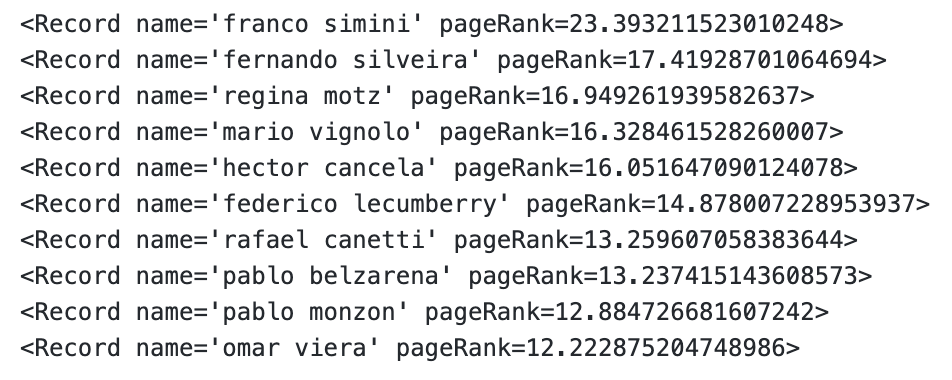
\includegraphics[width=\linewidth]{imagenes/pagerank.png}
	\caption{Top diez de personas con mayor puntaje por el algoritmo \textit{PageRank}.}
	\label{fig:page_rank}
\end{figure}


\subsubsection{Conclusiones del Análisis de Centralidad}
Presentados los distintos algoritmos que se pueden utilizar para obtener medidas de centralidad, se pueden identificar personas muy influyentes en la comunidad científica de la Facultad de Ingeniería. Hay individuos, como Fernando Silveira, Federico Lecumberry y Lorena Etcheverry, que son parte de más de un \textit{ranking} de nodos influyentes, lo que lleva a concluir que son actores importantes en esta base de datos.

\subsection{Detección de Comunidades}
Más allá de medir la importancia individual de los nodos, es posible analizar la estructura grupal de la red. El objetivo de la detección de comunidades es particionar el grafo en clusters o grupos de investigadores con una alta densidad de colaboraciones internas y conexiones más escasas con el exterior. Estos grupos suelen representar laboratorios, áreas temáticas o equipos de investigación consolidados.

Al igual que en el análisis de centralidad, los algoritmos de comunidad se ejecutan sobre la proyección del grafo de coautoría, \texttt{coauthor-graph}. En este trabajo se exploraron dos algoritmos populares de la librería GDS: Propagación de Etiquetas y Louvain.

\subsubsection{Propagación de Etiquetas (Label Propagation)}
El algoritmo de Propagación de Etiquetas (LPA) es un método heurístico y muy rápido para encontrar la estructura de comunidad "natural" de un grafo. Inicialmente, cada nodo recibe una etiqueta única (su propia comunidad). Luego, en iteraciones sucesivas, cada nodo adopta la etiqueta más frecuente entre sus vecinos. El proceso continúa hasta que se alcanza un consenso y las etiquetas de los nodos se estabilizan. La consulta para ejecutar este algoritmo es la siguiente:

\begin{sflisting}[style=sparql,caption= Detección de comunidades con Propagación de Etiquetas,label=codigo_lpa]
	CALL gds.labelPropagation.stream('coauthor-graph', {})
	YIELD nodeId, communityId
	RETURN gds.util.asNode(nodeId).normalized_name AS name,
		communityId AS community_id
\end{sflisting}

El resultado asigna un \texttt{communityId} a cada persona, agrupando a los investigadores en sus respectivos clusters de colaboración.

\subsubsection{Algoritmo de Louvain}
El método de Louvain es uno de los algoritmos de detección de comunidades más utilizados debido a su eficacia y escalabilidad. Su objetivo es optimizar una métrica llamada \textit{modularidad}, la cual mide la calidad de una partición del grafo. Una alta modularidad indica que la densidad de las conexiones dentro de las comunidades es significativamente mayor que la que se esperaría en una red aleatoria con la misma distribución de grados.

Aunque la consulta se muestra en su forma no ponderada, Louvain puede utilizar la propiedad \texttt{weight} de las relaciones (el número de trabajos en común) para que las colaboraciones más fuertes tengan más influencia en la definición de las comunidades, lo que suele producir resultados más significativos.

\begin{sflisting}[style=sparql,caption= Detección de comunidades con el algoritmo de Louvain,label=codigo_louvain]
	CALL gds.louvain.stream('coauthor-graph', {})
	YIELD nodeId, communityId
	RETURN gds.util.asNode(nodeId).normalized_name
	AS name, communityId
\end{sflisting}

Al igual que con Propagación de Etiquetas, esta consulta asigna un \texttt{communityId} a cada investigador, pero esta vez la partición del grafo se realiza según el criterio de máxima modularidad, identificando los grupos de colaboración más robustos. En la figura \ref{fig:comunidades} se muestran dos ejemplos de comunidades encontradas. Se pueden identificar en cada una de ellas docentes del Instituto de Ingeniería Eléctrica que son parte del mismo departamento. Además, se encuentran otros investigadores que forman parte de otros departamentos, generando una comunidad interdisciplinaria.

\begin{figure}[htb]
	\centering
	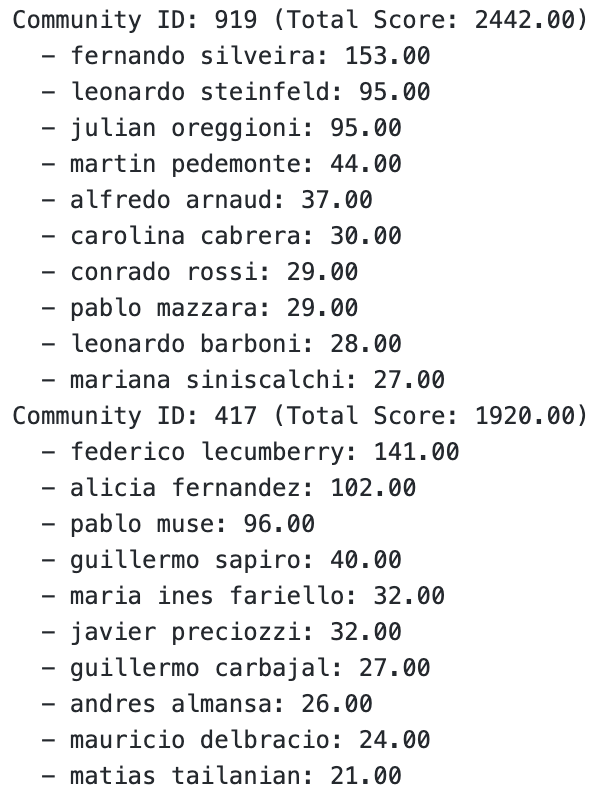
\includegraphics[width=\linewidth]{imagenes/comunidades.png}
	\caption{Ejemplo de dos comunidades encontradas con el Algoritmo de Louvain.}
	\label{fig:comunidades}
\end{figure}


\section{Conclusiones y Trabajo Futuro}
\label{conclusion}
Este proyecto demostró que el modelado de la producción académica de la Facultad de Ingeniería en una base de datos de grafos es una aproximación factible y potente. La integración de fuentes como Colibrí y OpenAlex en un único grafo resultó ser una solución eficaz para centralizar y conectar información, mientras que el uso del lenguaje de consulta \textit{Cypher} otorgó una gran flexibilidad para explorar relaciones complejas, como patrones de coautoría y vínculos temáticos, de una manera ágil e intuitiva.

El trabajo en su conjunto constituye una sólida prueba de concepto. Aunque el estudio se limitó a los individuos de la Facultad, la arquitectura del sistema está diseñada para crecer. Posibles líneas de trabajo futuro son: expandir el grafo para incluir a todos los investigadores de la Facultad e incorporar nuevas entidades como filiación para identificar colaboraciones interinstitucionales. Estos pasos permitirían transformar el prototipo actual en un recurso analítico de gran valor estratégico para la institución.

%\bibliographystyle{plainnat}
\bibliographystyle{IEEEtran}
\bibliography{final-article}


\end{document}